
\documentclass[spanish]{article}
\usepackage[utf8]{inputenc}
\usepackage[spanish]{babel}
\usepackage{graphicx}
\usepackage{float}
\usepackage{caption}
\usepackage{listings}

\title{Proyecto de Inteligencia Artificial}
\author{David Sánchez Iglesias}
\date{2023}

\begin{document}
\maketitle

\section{Introducci\'on}
En el presente proyecto se simula y estudia el comportamiento de un modelo de seguros de riesgo (Insurance Risk Model).
El objetivo es estudiar la evoluci\'on del capital de la firma de seguros.
Dicho problema se encuentra en el libro ``Simulation, Fifth edition'' de Sheldon M. Ross, en el cap\'itulo 7, ep\'igrafe 7.6, p\'agina 122.

\section{Problema}
Se tiene una compa\~n\'ia de seguros de riesgo con la cantidad de clientes que poseen un seguro de esta. Se tiene que se generan, contra la empresa, reclamaciones de acuerdo a un proceso de Poisson independiente, con una tasa com\'un $\lambda$, por una cantidad de dinero cuya distribuci\'on \textit{F} se conoce. Se tiene tambi\'en que los nuevos cliente firman para la obtenci\'on de un seguro de acuerdo a otro proceso independiente de Poisson, con tasa \textit{v}, y que cada uno de los asegurados se mantiene con la compa\~n\'ia por un tiempo cuya distribuci\'on es exponencial, con tasa $\mu$. Se sabe que cada asegurado paga a la compa\~n\'ia una cantidad de dinero fija \textit{c} por unidad de tiempo.
Empezando con una cantidad fija de clientes y un capital inicial, la compa\~n\'ia est\'a interesada en simular este sistema para saber si el capital de la firma siempre se mantiene no negativo todo el tiempo hasta un momento dado.

\section{Modelaci\'on del problema}
\subsection{Variables}
Para simular el sistema, se cre\'o la clase \textit{InsuranceRiskModel}, con todas las variables y procesos que se usar\'an durante la simulaci\'on.
Entre sus variables se encuentran:
\begin{itemize}
    \item \textit{time}: la unidad de tiempo en la que se encuentra el sistema en un momento dado.
    \item \textit{n\_pols}: el n\'umero de asegurados (policyholders) en un tiempo espec\'ifico.
    \item \textit{capital}: recoge el capital que posee la empresa en el tiempo actual.
    \item \textit{lost\_pols}: cantidad de asegurados que dejaron la empresa. Este valor aumenta con cada ciclo y al final recoge la totalidad de asegurados que dejaron la empresa durante toda la simulaci\'on.
    \item \textit{events\_queue}: un heap, una cola con prioridad que almacena los eventos y los ordena seg\'un el tiempo en el que les toca ser ejecutado.
    \item \textit{events}: diccionario que recoge los diferentes tipos de eventos junto a la funci\'on que los genera.
    \item \textit{pol\_list}: contiene los id de los asegurados que posee la empresa en una unidad de tiempo. Se actualiza con cada cambio que ocurre entre los asegurados, o sea, si aparece o se pierde un asegurado.
\end{itemize}
Para reiniciar las variables en caso de que se quiera ejecutar la simulaci\'on varias veces, se crearon otras variables de referencia:
\begin{itemize}
    \item \textit{limit\_time}: tiempo l\'imite, introducido por el usuario al crear la clase.
    \item \textit{pol\_pay}: lo que paga cada asegurado (\textit{c})
    \item \textit{starting\_capital}: el capital inicial
    \item \textit{initial\_n\_pols}: la cantidad inicial de asegurados que posee la empresa.
    \item \textit{current\_pol\_id}: para establecer un valor, un codigo de identificaci\'on a cada asegurado. 
\end{itemize}
El resto de las variables tienen como objetivo almacenar las tasas de los diferentes procesos aleatorios as\'i como las funciones para la generaci\'on de los valores aleatorios y al almacenamiento de estad\'isticas recogidas durante el proceso.

\section{Flujo del programa}
La clase cuenta con tres m\'etodos principales:
\begin{itemize}
    \item \textit{run}: se encarga de sacar los eventos de la cola, producir los cambios que estos conllevan al sistema y actualizar el tiempo. Solo para si la cola est\'a vac\'ia (lo cual significa que ya no quedan eventos en lo que resta de tiempo) o si se llega al tiempo l\'imite establecido por el usuario.
    \item \textit{initialize}: restablece los valores de todas las variables de lo simulaci\'on a sus valores iniciales.
    \item \textit{simulate}: ejecuta la cantidad de simulaciones que se le pasaran como argumento a la funci\'on.
\end{itemize}
\section{Resultados y experimentos}
Se escogieron los siguientes valores para las pruebas:
\begin{lstlisting}[language=Python]
    model = InsuranceRiskModel(
        new_pol_rate=20,           # 15 nuevos clientes/mes
        lost_pol_rate=0.05,        # 5% de clientes se pierden
        starting_capital=1_00,
        starting_policy_holders=500,
        pol_time_fun= policyholder_time_in_the_firm, 
        next_claim= new_claim, 
        claim_rate= 5,
        limit_time=120,             # 120 meses
        pol_pay=150                 # $150 por poliza/mes
    )
\end{lstlisting}

Se realizaron varias pruebas y gr\'aficos para estudiar el comportamiento del sistema y se observ\'o un resultado interesante.
Acontinuaci\'on se muestra un gr\'afico que ilustra c\'omo cambia la variable objetivo con el paso del tiempo:
\begin{figure}[H]
    \centering
    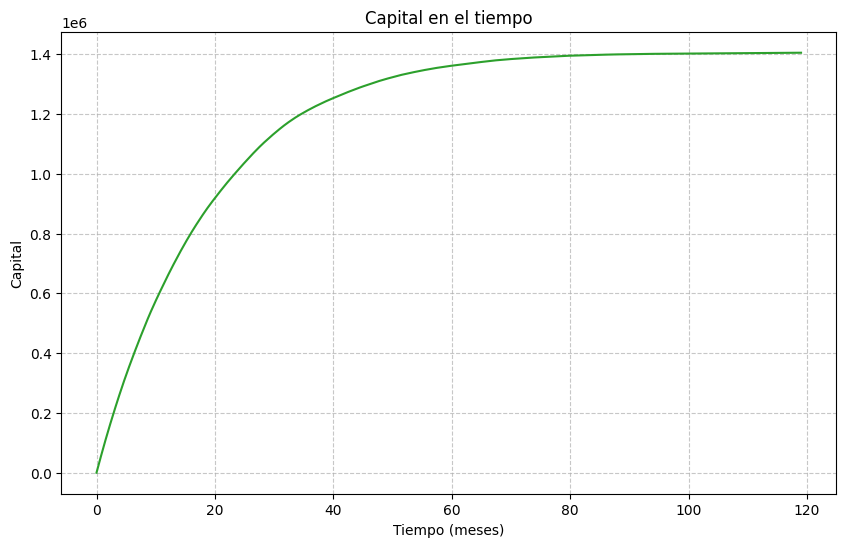
\includegraphics[scale=0.5]{capital_tiempo.png}
    \caption{Capital por unidad de tiempo}
    \label{fig:Capital por unidad de tiempo}
\end{figure}
En la figura claramente se ve que el capital de la empresa nunca es negativo, sin embargo tiende a estabilizarse hasta casi no variar.
La raz\'on detr\'as de este comportamiento se debe en parte al flujo de asegurados que entran y salen de la empresa.
%Insertar imagen
\begin{figure}[H]
    \centering
    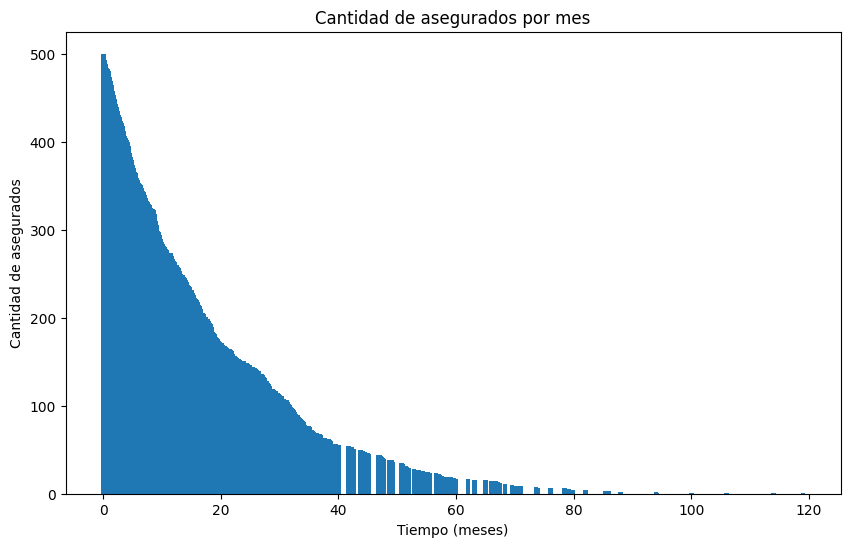
\includegraphics[scale=0.5]{cant_asegurados.png}
    \caption{Cantidad de asegurados por unidad de tiempo}
    \label{fig:Cantidad de asegurados por unidad de tiempo}
\end{figure}
Esta gr\'afica muestra c\'omo hay una disminuci\'on clara de la cantidad de asegurados a medida que pasa el tiempo.
Ya que, seg\'un los datos con los que se cuenta, el dinero que pagan los asegurados es la \'unica fuente de ingresos de la empresa, no sorprende que el capital se comporte de esa manera.
De hecho, al realizar m\'as simulaciones queda en evidencia que esta situaci\'on siempre ocurre, y la siguiente figura as\'i lo muestra:
\begin{figure}[H]
    \centering
    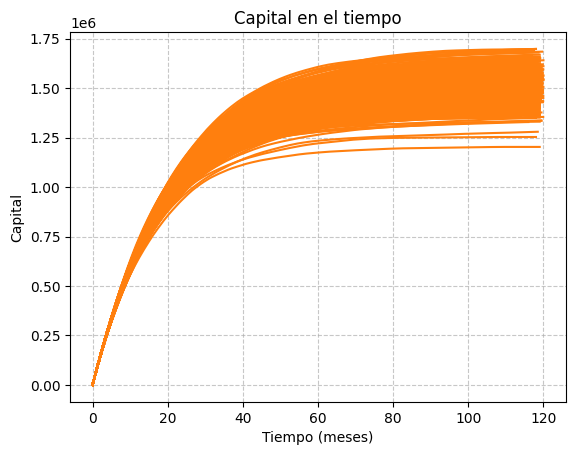
\includegraphics[scale=0.5]{capital_tiempo_mil_sim.png}
    \caption{Capital por unidad de tiempo, en 1000 simulaciones}
    \label{fig:Capital por unidad de tiempo, en 1000 simulaciones}
\end{figure}
Esta figura muestra que el capital parece comportarse igual, como si distribuyera de una forma espec\'ifica.

\subsection{Hip\'otesis: El capital de la empresa distribuye de acuerdo a una funci\'on.}

A vista, la gr\'afica se asemeja mucho a una exponencial negativa, una funci\'on log\'istica o una logar\'itmica.
Se realiz\'o entonces un ajuste de modelos para verificar si alguna de estas describ\'ian el comportamiento del capital.\\
F\'ormulas probadas:\\
\begin{itemize}
    \item Log\'istica: $C(t) = \frac{L}{1 + e^{-k\left(t - t_0\right)}}$
    \item Exponencial negativa: $C(t) = L(1 - e^{-kt})$
    \item Logar\'itmica: $C(t) = a + b\ln(t)$
\end{itemize}

El resultado:
\begin{figure}[H]
    \centering
    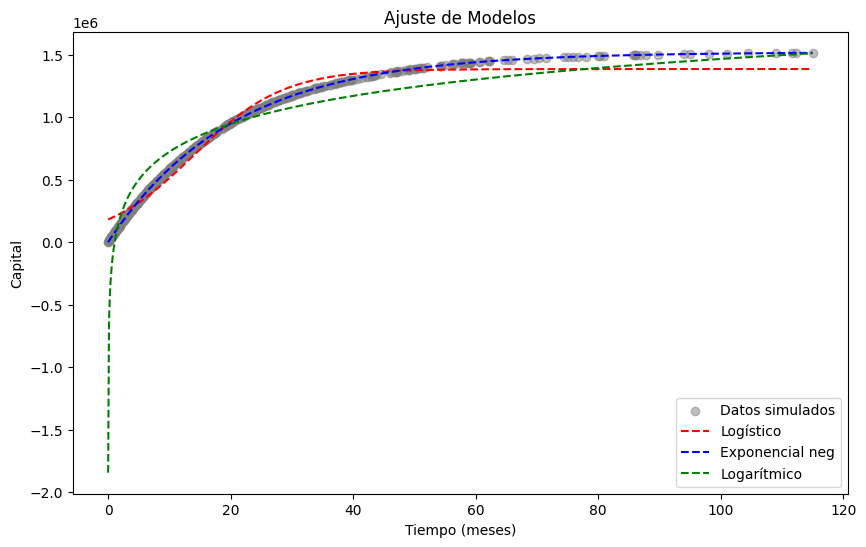
\includegraphics[scale=0.5]{ajustes_de_modelos.png}
    \caption{Ajustes de diferentes modelos a los datos}
    \label{fig:Ajustes de los modelos a los datos}
\end{figure}
Evidentemente la exponencial negativa parece ser la que m\'as se ajusta, seguida de la log\'istica, mientras la logar\'itmica se desv\'ia.
Una \'ultima comprobaci\'on gr\'afica, esta vez con los residuales, nos muestra que, en efecto, la exponencial es la que parece ajustarse m\'as al comportamiento de los datos extra\'idos al encontrarse todos sus residuos sumamente cercanos a cero.
\begin{figure}[H]
    \centering
    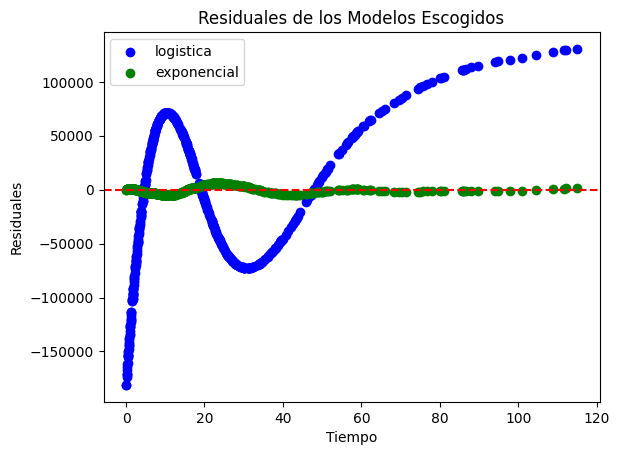
\includegraphics[scale=0.5]{residuales.png}
    \caption{Residuales de la log\'istica y la exponencial}
    \label{fig:Residuales de la log\'istica y la exponencial}
\end{figure}
Para comprobarlo se realiz\'o el c\'alculo del error medio cuadr\'atico.
\begin{equation}
    MSE(F) \equiv E_F[(g(X_1,X_2,\dots X_n) - \theta(F))^2]
\end{equation}
Dicho resultado se normaliz\'o con la varianza para una mejor visualizaci\'on. 
Como resultado, el error da aproximadamente 0.00505, lo que se traduce en un 0.005\% de la varianza de los datos. En otras palabras, la funci\'on exponencial propuesta describe el comportamiento del capital durante la simulaci\'on. Se puede considerar que esta funci\'on sirve como funci\'on de distribuci\'on para la variaci\'on del capital de esta empresa.
\section{Conclusi\'on}
Con los datos proporcionados y los valores establecidos para la simulaci\'on, el capital nunca ser\'a negativo pues su funci\'on de distribuci\'on (la exponencial reci\'en estudiada) nunca es negativa.


\end{document}